

%----------------------------------------------------------------------------------------
%	PART
%----------------------------------------------------------------------------------------


\part{Capítulo seis}
\graphicspath{ {img/ch6/}, {img/} }




%----------------------------------------------------------------------------------------
%	CHAPTER 6
%----------------------------------------------------------------------------------------

\chapterimage{ima2} % Chapter heading image


\chapter{Gradientes}

%\begin{center}
%	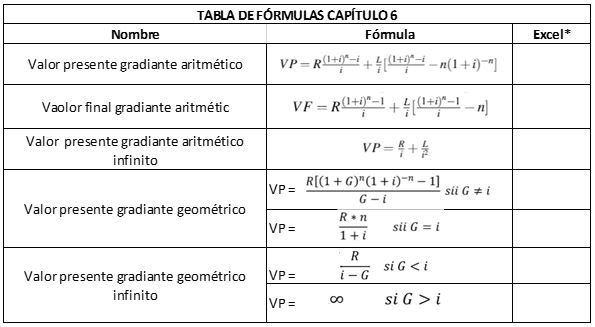
\includegraphics[height=5.5cm]{TE6.JPG}
%\end{center}

\section{{Fórmulas del capítulo}}


\begin{center}
\begin{tabular}{ |p{6.8cm}|p{5cm}| p{3.2cm}|}
\hline 
\rowcolor{orange!50} 
\begin{center}\textbf{Fórmula}\end{center} & \begin{center}\textbf{Nombre}\end{center} & \begin{center}\textbf{Excel}\end{center}   \\ \hline                        


$VP = R  \frac{1-(1 + i)^{-n}}{i} + \frac{L}{i}[ \frac{1-(1 + i)^{-n}}{i} - n(1 + i)^{-n} ]$\hspace{35 pt} & Valor presente gradiante aritmético & VNA(i;R1;R2;R3;...)\\ \hline 


$VF = R\frac{(1+i)^n-1}{i} + \frac{L}{i}[\frac{(1+i)^n-1}{i}-n]$ \hspace{35 pt} & Valor futuro gradiante aritmético  
 & - \\  \hline 


$VP = \frac{R}{i} + \frac{L}{i^2}$ \hspace{35 pt} & Valor  presente gradiante aritmético infinito		
 & - \\ \hline 

$R_{n} = R_{1} + (n-1)L$ \hspace{35 pt} & Valor último flujo de un gradiente aritmético		
 & - \\ \hline  
 
 $VP = R  \frac{(1 + g)^n (1 + i)^{-n}-1}{g - i} $ \hspace{35 pt} & Valor presente gradiante geométrico si  $g \neq i$ &  
 - \\ \hline 

$VP = \frac{R n}{1 + i}$ \hspace{35 pt} & Valor presente gradiante geométrico si g = i	 &  VNA(i;R1;R2;R3;...)\\ \hline

$R_{n} = R_{1}(1+g)^{n-1}$ \hspace{35 pt} & Flujo n de un gradiente geométrico & - \\ \hline 

$VP = \frac{R}{1 - g} $ \hspace{35 pt} & Valor presente gradiante geométrico infinito si g < i 	
 &  VNA(i;R1;R2;R3;...) \\ \hline 

 $VP = \infty $ \hspace{35 pt} & Valor presente gradiante geométrico infinito si $g \geq i$ & - \\ \hline 


$VF = R  \frac{(1 + g)^n - (1 + i)^n}{g - i} $ & Valor futuro gradiente geométrico si $g \neq i$  & - \\ \hline 

$VF = Rn(1 + i)^{n-1} $ & Valor futuro gradiente geométrico si $g = i$  & - \\ \hline 

\end{tabular}
\end{center}


\section{Introducción}


Debido a la inflación, se observa que casi todos los renglones de la economía van aumentando de precios, por esta razón, es necesario elaborar modelos matemáticos que ajustándose a los índices de inflación puedan compensar los efectos erosionantes en el dinero a través del tiempo, entre los modelos matemáticos que pueden suplir esta necesidad están los gradientes.\\

\subsection{Definición}

Un gradiente es una serie de ingresos o egresos que cumplen con las siguientes condiciones:\\
\begin{enumerate}
	\item Todos los ingresos o egresos cumplen con una ley de formación.
	\item Los ingresos o egresos se efectúan a iguales intervalos de tiempo.
	\item Todos los ingresos o egresos se trasladan al principio o al final con la misma tasa de interés.
	\item El número de ingresos o egresos es igual al número de períodos.\\
\end{enumerate}

La ley de formación, de la que habla la primera condición, puede ser de varias clases, sin embargo, las más utilizadas son: la que corresponde al gradiente lineal o aritmético y la que corresponde al gradiente geométrico.\\

Las series uniformes de tiempo, vienen a ser un caso particular de los gradientes, en el cual, el crecimiento es cero, lo que hace que todos los ingresos o egresos sean de igual valor, por tal motivo el manejo de los gradientes es similar al manejo de las series uniformes de tiempo.\\

Las otras tres leyes son las mismas de las series uniformes.\\

\section{Gradiente aritmético (VP, VF, L, i, n)}

En el gradiente aritmético cada ingreso o egreso es igual al anterior, más una constante L; si esta constante es positiva, el gradiente será creciente, si la constante es negativa, el gradiente sera decreciente. Obviamente si L = 0 todos los ingresos o egresos son iguales y la serie se convierte en una serie uniforme. Como en un gradiente todos los ingresos o egresos son de diferente valor, será necesario distinguir dicho ingreso o egreso de otro y por eso al primer ingreso o egreso lo representaremos por $R_{1}$; el segundo ingreso o egreso por $R_{2}$ y así sucesivamente, el último ingreso o egreso lo representaremos por $R_{n}$. De acuerdo a la definición de gradiente lineal se tendrá:\\

$R_{2} = R_{1} + L$\\
$R_{3} = R_{2}  + L  = R_{1} + 2L$\\
... ... ... ... \\
$R_{n} = R_{1} + (n-1)L$\\
De lo anterior se deduce que la fórmula del último término será:\\
$R_{n} = R_{1} + (n-1)L$ \hspace{35 pt} \textit{Valor último flujo de un gradiente aritmético}\\

\textbf{Ejemplo 1}
Hacer la gráfica de un gradiente aritmético de 6 ingresos anuales vencidos con primera cuota de \$100.
\begin{itemize}
	\item a. Crecimiento de \$25
	\item b. Decreciente en \$25
\end{itemize}

\clearpage

\textbf{Solución:}

\begin{itemize}
	\item a.Crecimiento de \$25\\
	figura(a)\\
	%imagen 1
  %  \begin{figure}[h]
	\begin{center}
	   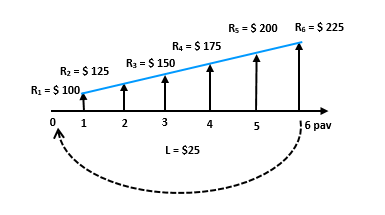
\includegraphics[height=4.5cm]{6_1}			
	\end{center}	
%\end{figure}
	
	\item b.Decrecimiento en \$25\\
	figura(b)\\
	%imagen 2
	\begin{center}
		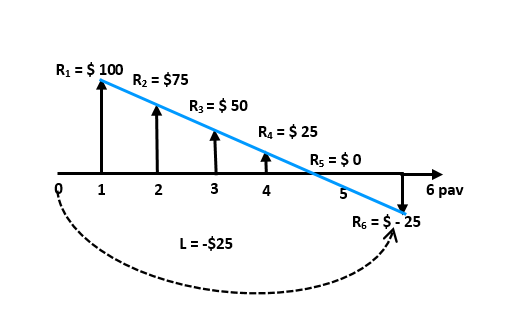
\includegraphics[height=4.5cm]{6_2}
	\end{center}

\end{itemize}

Observese en la fígura (b) que, en el período 5, el ingreso es cero y que,en el período 6, el valor del ingreso viene a ser -\$25, lo cual se representa un egreso de -\$25.

\section{Fórmula del valor presente del gradiente aritmético (VP, L, i, n)}
%imagen 3
\begin{center}
	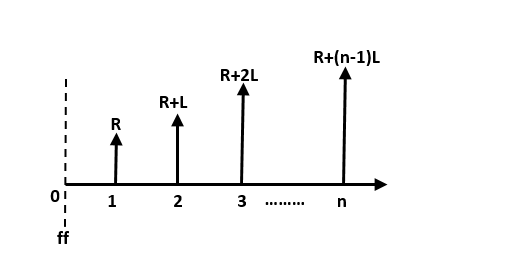
\includegraphics[height=4.5cm]{6_3}
\end{center}
En igual forma como se hizo con las series uniformes vencidas, planteamos la ecuación de valor, trasladando cada uno de los ingresos o egresos a la fecha focal, usando la tasa periódica i vencida; entonces:\\\\
$VP=R\frac{(1+i)^n-i}{i}+\frac{L}{i}[\frac{(1+i)^n-i}{i}-n(1+i)^{-n}]$\hspace{35 pt} \textit{Valor presente de un gradiente aritmético}\\
	
	En la fórmula anterior esta R pero sin indicar cuál de las cuotas es, sin embargo en la deducción de la fórmula hemos trabajado con base en que R es el primer ingreso o egreso. En consecuencia cuando cualquier fórmula aparezca R sin indicar cuál es, deberá asumirse que se trata de la primera cuota.\\
	
	\textbf{Ejemplo 2}\\
	Hallar el valor presente con un interés del 5\% periódico año vencido de la siguiente gráfica:\\
	
	%imagen 3
	\begin{center}
		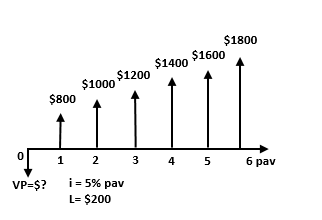
\includegraphics[height=4.5cm]{6_4}
	\end{center}
	
	\textbf{Desarrollo:}
	\begin{itemize}
		\item a.Diagrama de flujo\\
		%imagen 3.1
		\begin{center}
			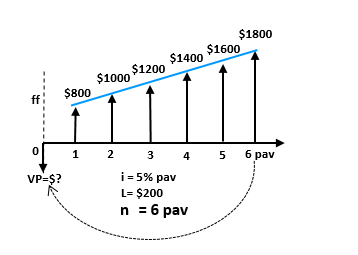
\includegraphics[height=5.0cm]{6_4_2}
		\end{center}
		\item b. Definición de variables\\		
			R = \$800\\
			i=5\% pav\\
			n=6\ pav\\		
			L =\$ 200\\			
			VP = \$?\\
		\item c. Declaración de fórmula\\\\
		$VP=R\frac{(1+i)^n-i}{i}+\frac{L}{i}[\frac{(1+i)^n-i}{i}-n(1+i)^{-n}]$ \hspace{35 pt} \textit{Valor presente de un gradiente aritmético}\\
		\item d.Reemplazando en la fórmula\\
		$VP=\$800\hspace{5 pt} \frac{1-(1+0,05)^{-6}}{0,05}+\frac{\$200}{0,05}[\frac{1-(1+0,05)^{-6}}{0,05}-6 \hspace{3 pt}(1+0,05)^{-6}]$ \hspace{35 pt} \textit{Ecuación de valor}\\
		VP =  \$6.454,15\\
		\item e. Respuesta:\\
		El valor presente es de \$6.454,15 COP\\
	\end{itemize}
	
	\textbf{Ejemplo 3}\\
	Hallar el valor presente de la siguiente serie con una tasa del 5\% periódica año vencido.\\
	
	%imagen 4
	\begin{center}
		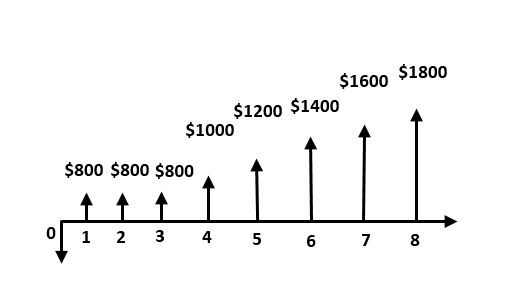
\includegraphics[height=4.0cm]{6_5}
	\end{center}
	
	\textbf{Desarrollo}
	\begin{itemize}
		\item a. Diagrama de flujo
		\begin{center}
			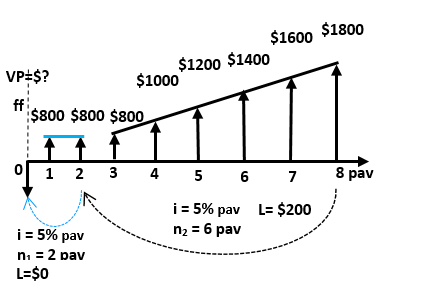
\includegraphics[height=4.5cm]{6_5_2}
		\end{center}
		
        \textbf{(a) Primera forma para resolver el ejercicio:}\\
        Entonces, el VP es igual a la suma del VP de la serie uniforme vencida en donde R=\$800; $n_{1}$=2 pav; i=5\% pav; Más: el VP del gradiente aritmético, en donde L=\$200; $n_{2}$=6 pav, del período 8 al 2; i =5 \% pav en la "fecha focal parcial en n=2 pav; trasladada por la fórmula $P=F(1+i)^{-n}$ del período 2 al período 0. \\
        \\
        \begin{center}
			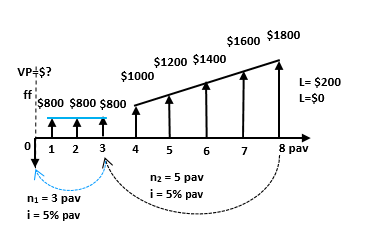
\includegraphics[height=4.5cm]{6_5_3}
		\end{center}
		
        \textbf{(b)Segunda forma para resolver el ejercicio:}\\
        El VP es igual a la suma del VP de la serie uniforme en donde R=\$800; $n_{1}$=3 pav; i=5\% pav; Más: el VP del gradiente aritmético, en donde L=\$200; $n_{2}$=5 pav; i =5 \% pav en la "fecha focal parcial de n=3 pav; trasportada por la formula $P=F(1+i)^{-n}$\ del período 3 al período 0.\\
				
		\item b. Declaración de variables \\
		Para la primera forma de resolver el ejercicio: \\
		R= \$800\\
		i = 5\% pav\\
		L = \$200\\
		$n_{1}$ = 2pav\\
		$n_{2}$ = 6pav \\
		VP=\$?\\
		Para la segunda forma de resolver el ejercicio:\\
	    R= \$800\\
		i = 5\% pav\\
		L = \$200\\
		$n_{1}$ = 3pav\\
		$n_{2}$ = 5pav \\
		VP=\$?\\
		\item c. Declaración de fórmulas\\
$VP=R\frac{(1+i)^n-i}{i}+\frac{L}{i}[\frac{(1+i)^n-i}{i}-n(1+i)^{-n}]$\hspace{3 pt} \textit{VP del gradiente aritmético}\\
		$VP=R\hspace{3 pt}\frac{(1-(1+i)^{-n})}{i}$ \hspace{10 pt} \textit{Valor presente de una serie uniforme vencida}\\
        $P=F(1+i)^{-n}$ \hspace {35 pt} \textit{Valor presente dado un valor futuro}\\
        
		\item d. Reemplazando la fórmula\\
		Primera forma: podemos considerar que el gradiente se inicia en el período 2; entonces su primer pago será de \$800 (el que está en 3); los otros pagos de \$800 ubicados en 1 y 2 forman una serie uniforme vencida:\\
		
		La fecha focal es en n=0.
        Entonces el VP= a la suma del VP de la serie uniforme en donde R=\$800; n=2 pav; i=5\% pav; Más: el VP del gradiente aritmético, en donde L=\$200; n=6 pav; i =5 \% pav en la "fecha focal parcial de n=2 pav; trasportada por la formula $P=F(1+i)^{-n}$ del período 2 al período 0. \\
        
		$VP = \$800 \hspace {3 pt} \frac{1-(1+0.05)^{-2}}{0,05} + [800\frac{1-(1+0.05)^{-6}}{0,05}+\frac{200}{0,05}[\frac{1-(1+0.05)^{-6}}{0,05}-6*(1+0,05)^{-6}]](1+0,05)^{-2}$ \hspace{35 pt} \textit{Ecuación de valor para ff en el período 0}\\
		
		Segunda forma: podemos suponer que el gradiente empieza en el periodo 3; así su primer pago será de \$1000, y tendrá 5 periodos.\\
		
		$VP = \$800 \hspace {3 pt} \frac{1-(1+0.05)^{-3}}{0,05}+[1000\frac{1-(1+0.05)^{-5}}{0,05}+\frac{200}{0,05}[\frac{1-(1+0.05)^{-5}}{0,05}]*(1+0,05)^{-3}$ \\ \textit{Ecuación de valor}\\
		\item e. Respuesta\\
		Luego el valor presente de la serie es \$7.342 COP
	\end{itemize}
	
	\section{Fórmula del valor final del gradiente aritmético (VF, L, i, n)}
	
	Para hallar el valor final, basta tomar el valor presente y multiplicarlo por $(1+i)^n$, así:\\
	$F= P(1+i)^n$ \hspace{35 pt} \textit{Valor futuro dado un valor presente}
	
	\vspace{2mm}
	Haciendo las operaciones respectivas y simplificando se concluye que:
	
	$VF = R\frac{(1+i)^n-1}{i} + \frac{L}{i}[\frac{(1+i)^n-1}{i}-n]$ \hspace{35 pt} \textit{Valor final del gradiente aritmético}\\
	
	\textrm{Observación} nuevamente hacemos énfasis en que R representa la primera cuota del gradiente.
	
	\textbf{Ejemplo 4}\\
	Hallar el monto o el valor final VF del siguiente flujo de caja que renta una tasa del 15\% periódica año vencido. \\
	\textbf{Observación:} los 2 últimos valores son negativos.\\
	%imagen 5
	\begin{center}
		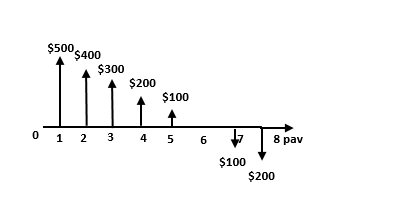
\includegraphics[height=4.5cm]{6_6}
	\end{center}
	
	\textbf{Desarrollo}
	\begin{itemize}
		\item a. Diagrama de flujo:
		%imagen 5
		\begin{center}
			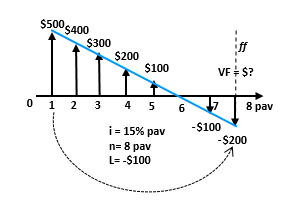
\includegraphics[height=5.0cm]{6_6_2}
		\end{center}
		\item b. Declaracion de variables\\
		R=\$500\\
		i= 15\% pav.\\
		n= 8 pav\\
		L=-\$100\\
		\item c. Declaración de fórmulas\\
		$VF = R\frac{(1+i)^n-1}{i} + \frac{L}{i}[\frac{(1+i)^n-1}{i}-n]$ \hspace{35 pt} \textit{Valor final de gradiente aritmético}\\
		\item d. Desarrollo matematico\\
		$VF = \$500\frac{(1+0,15)^8-1}{0,15} + \frac{-\$100}{0,15}[\frac{(1+0,15)^8-1}{0,15}{-8}]$ \hspace{30 pt} \textit{Ecuación de valor }\\
		\item e. Respuesta\\
		Luego el monto es de \$3.045 COP\\
		
		\section{Amortización con cuota creciente}
		
		Debido a las altas tasas de inflación, en muchos países se ha impuesto la moda de utilizar una cuota creciente en los sistemas de amortización, lo que ha impulsado el desarrollo de nuevas técnicas.\\
		
		\textbf{Ejemplo 5}\\
		a. Elaborar una tabla de amortización  con cuota lineal creciente de \$12.000 para la suma de \$100.000 en 4 pagos anuales y una tasa del 8\% periódica año vencido.\\ 
        b. una tabla amortización una cuota lineal decreciente de \$12.000.\\
        
		\begin{itemize}
			\item A. Crecimiento lineal de la cuota de \$12.000
			\item B. Decremento lineal de la cuota de \$12.000\\
		\end{itemize}
		
		\textbf{Solución}\\
		\begin{itemize}
			\item a. Diagrama de flujo para una tabla de amortización de una cuota de pago creciente de \$12.000:\\
			%imagen 6
			\begin{center}
				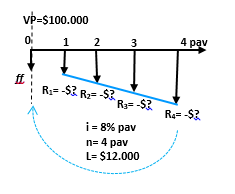
\includegraphics[height=5.0cm]{6_7}
			\end{center}
			La fecha focal se fija en el período 0.
            Una tabla de amortización  muestra, período a período, la forma como se va cancelando mediante cuotas crecientes de una deuda. Para construir la tabla de amortización, primero se calcula la cuota del pago a partir de la forma del VP del gradiente lineal vencido L. Luego se registra el pago creciente, $R_{1} = Ro+Lo$, en la columna cuatro de la tabla de cinco columnas, compuesta de: período, saldo de la deuda, Intereses, pago creciente y amortización. La ultima fila de la columna saldo de la deuda acumulado debe ser igual a \$0.\\

			\item b. Declaración de variables\\
			VP = \$100.000\\
			R = \$?\\
			n = 4 pav\\
			L = \$12000\\
			i = 8\% pav\\
			\item c. Declaración de fórmulas
			
			\vspace{2mm}
			
			$VP = R	\frac{1-(1+i)^{-n}}{i}+\frac{L}{i}[\frac{1-(1+i)^-{n}}{i}- n(1+i)^{-n}]$ \hspace{5 pt} \textit{Valor presente del gradiente aritmético}\\
			$R_{n} = R_{1} + (n-1)L$\hspace{10 pt} \textit{Valor último flujo de un gradiante aritmético}\\
			
			\clearpage
			
			\item d. Desarrollo matemático\\
			$\$100.000 = R	\frac{1-(1+0,08)^{-4}}{i}+\frac{1200}{0,08}[\frac{1-(1+0,08)^{-4}}{0,08}- 4(1+0,08)^{-4}]$ 
			\\
			\textit{Ecuación de valor para la ff en el período 4}\\
			\item e. Solución:\\
			Despejando R se obtiene que : $R_{1} = \$13.344,56$\\
			Las demás cuotas se pueden calcular con la fórmula del último término del gradiente lineal o aritmético\\
			$R_{n} = R_{1} + (n-1)L$\\
			$R_{2} = 13.344,56 + 12000 = \$25.344,56$\\
			$R_{3} = 13.344,56 +2 (12000) = \$37.344,56$\\
			$R_{4} = 13.344,56 +3 (12000) = \$49.344,56$\\
		\end{itemize}
		
		Con los anteriores datos podemos elaborar la tabla de amortización en la misma forma como se trabajo con las series uniformes\\
		
		%tabla1
		%imagen 6
		%\begin{center}
		%	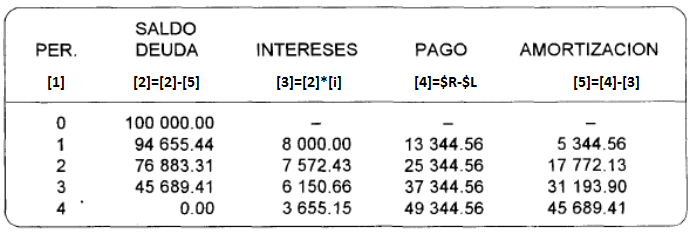
\includegraphics[height=4.0cm]{6_8}
		%\end{center}
		
    \begin{center}
        \begin{tabular}{|p{1cm}|p{2cm}|p{2cm}|p{2cm}|p{3cm}|}
        \hline 
        \rowcolor{white!50}
            \textbf{n\ (1)} & \textbf{Saldo Deuda (2)=(2)-(5)} & \textbf{Intereses  (3)=(2)(i)}& \textbf{Pago\ (4)=\$R-\$L }& \textbf{Amortización  (5)=(4)-(3)} \\ \hline                        
 
            0 & \$100.000,00 & --------- & --------- & ---------\\ \hline 
            1 & \$7.845,30  & \$1.000,00  & \$3.154,70  & \$2.154,70 \\ \hline
            2 & \$5.475,13  & \$784,53  & \$3.154,71  & \$2.370,17 \\ \hline
            3 & \$2.867,94 & \$547,51  & \$3.154,72 & \$2.607,19 \\ \hline
            4 & \$0,03  & \$286,79  & \$3.154,73  & \$2.867,91 \\ \hline

 
\end{tabular}
\end{center}
		
		\begin{flushleft}
             \textbf{Solución literal b.}\\
        \end{flushleft}
        \begin{itemize}
		   \item a. Diagrama de flujo para una tabla de amortización de una cuota de pago decreciente de \$12.000:
			%imagen 7
			\begin{center}
				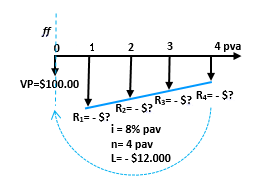
\includegraphics[height=5.0cm]{6_9}
			\end{center}
			\item b.Declaración de variables\\
			VP = \$100.000\\
			R = \$?\\
			n = 4 pav\\ L = -\$12.000\\ i=8\% pav.
			\item c. Declaración de fórmulas\\
			$VP = R	\frac{1-(1+i)^{-n}}{i}+\frac{L}{i}[\frac{1-(1+i)^{-n}}{i}- n(1+i)^{-n}]$ \hspace{10 pt} \textit{Valor presente de gradiente aritmético}\\
			$R_{n} = R_{1} + (n-1)L$\hspace{20 pt} \textit{Valor último flujo de un gradiante aritmético}\\
			\item d. Desarrollo matemático\\
			$\$100.000 = R	\frac{1-(1+0,08)^{-4}}{i}+\frac{-1200}{0,08}[\frac{1-(1+0,08)^{-4}}{0,08}- 4(1+0,08)^{-4}]$ \\ \textit{Ecuación de valor para la ff en el período 4}\\
			\item e. Justificación\\
			Se obtiene que $R_{1} = \$47.039,60$\\
			%imagen 7
			%\begin{center}
			%	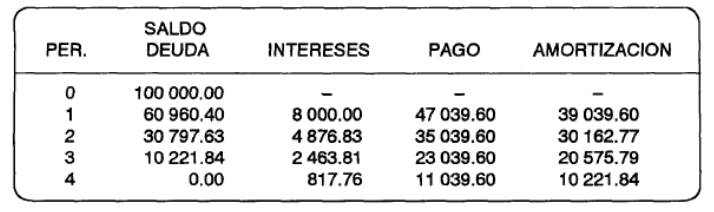
\includegraphics[height=4.0cm]{6_10}
			%\end{center}
			
\begin{spacing}{1.1}
    \begin{center}
        \begin{tabular}{|p{1cm}|p{2cm}|p{2cm}|p{2cm}|p{3cm}|}
        \hline 
        \rowcolor{white!50}
            \textbf{n\ (1)} & \textbf{Saldo Deuda (2)=(2)-(5)} & \textbf{Intereses  (3)=(2)(i)}& \textbf{Pago\ (4)=\$R-\$L }& \textbf{Amortización  (5)=(4)-(3)} \\ \hline                        

            0 & \$100.000,00 & --------- & --------- & ---------\\ \hline 
            1 & \$60.960,40  &\$ 8.000,00  & \$47.039,60  & \$39.039,60 \\ \hline
            2 & \$30.797,63  &\$ 4.876,83  & \$35.039,60  & \$30.162,77 \\ \hline
            3 & \$10.221,84 & \$2.463,81  & \$23.039,60 & \$20.575,79 \\ \hline
            4 & \$0,00  & \$817,76  & \$11.039,60  & \$10.221,84 \\ \hline

 
\end{tabular}
\end{center}
\end{spacing}
		\end{itemize}
	\end{itemize}
	
	\section{Gradiente aritmético infinito}
	Igual que en las series uniformes vencidas, solo tiene sentido el valor presente de un gradiente 	infinito. Su principal aplicación es el cálculo del costo del capital, tema que se discutirá en un capitulo posterior
	
	$VP = \frac{R}{i} + \frac{L}{i^2}$ \hspace{35 pt} \textit{Valor presente de un gradiente aritmético infinito}\\
	
	\textbf{Ejemplo 6}\\
	Calcular el valor presente de una serie infinita de egresos que crecen en \$10, si el primer egreso es de \$200 y la tasa es del 3\% periódica mes vencido.\\
	
	\textbf{Solución}\\
	\begin{itemize}
		\item a. Diagrama de flujo:\\
		\begin{center}
			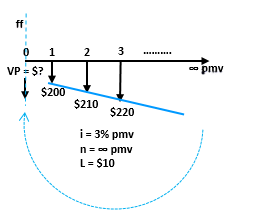
\includegraphics[height=5.5cm]{6_11}
		\end{center}
		
		\clearpage
		
		\item b. Declaración de variables\\
		n = $\infty$ \hspace{3 pt} pmv\\ 
		i = 3\% pmv\\ 
		L = \$10\\
		VP = \$?\\
        \item c. Declaración de fórmulas\\
        $VP = \frac{R}{i} + \frac{L}{i^2}$ \hspace{35 pt} \textit{Valor presente de un gradiente aritmético}\\
        \item d. Desarrollo matemático\\
		$VP = \frac{200}{0,03} + \frac{10}{0,03^{2}} = \$17.777,78$ \hspace{35 pt} \textit{Ecuación de valor }\\
		\item e. Solución\\
		Esto significa que si colocamos \$17.777,78 al 3\% pmv, podremos pagar \$200 al final del primer período, \$210 al final del segundo período, \$220 al final del tercer período y así sucesivamente.
	\end{itemize}
	
	\section{Gradiente geométrico}
	Un gradiente geométrico es una serie de ingresos o egresos, en la cual, cada ingreso o egreso es igual al anterior, multiplicado por una constante que representaremos por (1+g), Si g es positivo el gradiente será creciente, si g es negativo el gradiente será decreciente y, si g = 0 el gradiente se convierte en una serie uniforme vencida.\\
	
	En un gradiente geométrico, el primer paso será: $R_{1}$\\
	El segundo ingreso o egreso $R_{2} = R_{1}(1+g)$\\
	El tercer ingreso o egreso $R_{3} = R_{2}(1 + g) = R_{1}(1 + g)^{2}$\\
	El último ingreso o egreso entonces: $R_{n} = R_{n-1}(1+g) = R_{1}(1+g)^{n-1}$\\
	$R_{n} = R_{1}(1+g)^{n-1}$ \hspace{35 pt} \textit{Flujo n de un gradiente geométrico}\\
	Dónde:\\
	$R_{1} = Primer \hspace{5 pt} ingreso \hspace{5 pt} o \hspace{5 pt} egreso \hspace{5 pt} vencido$\\
	g = tasa de crecimiento de los ingresos o egresos\\
	
	\section{Fórmula del valor presente del gradiente geométrico}
	%formula
	\begin{center}
	\fontsize{13}{13}\selectfont
			$P = \left \{ \begin{matrix}\frac{R(1+g)^{n}(1+i)^{-n}}{g-i}& \mbox{si }g\mbox{ diferente de i}
\\ \frac{R(n)}{1+i} & \mbox{si }g\mbox{ igual a i}\end{matrix}\right.$
	\end{center}
	Donde\\
	n = número de períodos\\
	R = el primer ingreso o egreso efectuado\\
	i = tasa periódica vencida\\
	g = porcentaje de crecimiento de los pagos(en decimal)\\
	
	\textbf{Ejemplo 7:}\\
	Hallar el valor presente de 10 egresos anuales, si el primer egreso es de \$5.000 y cada egreso subsiguiente crece un 20\%. Suponga una tasa del 20\% períodica anual vencida.
	
	\clearpage
	
	\textbf{Solución:}
	\begin{itemize}
		\item a. Diagrama de flujo:
		%imagen formula
		\begin{center}
			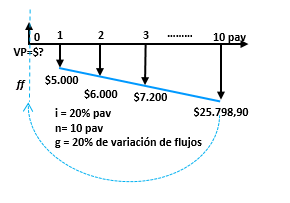
\includegraphics[height=4.5cm]{6_13}
		\end{center}
		\item b. Declaración de variables\\
		R = \$5.000\\ n = 10 pav\\ i= 20\% pav\\ g=20\% de incremento entre flujos, valor igual a la magnitud de la tasa de interés períodica\\ VP=\$?\\
		\item c. Declaración de fórmulas\\
		$VP = \frac{(R)(n)}{1+i}$ \hspace{35 pt} \textit{Valor presente de un gradiente geométrico para i = g, en valor absoluto}\\
		$R_{n} = R_{1}(1+g)^{n-1}$ \hspace{35 pt} \textit{Valor del flujo n de un gradiente geométrico}\\
		\item d. Desarrollo matemático\\
		$VP = \frac{(\$5000)(10)}{1+0,2} = \$41.666,67$ \hspace{35 pt} \textit{Ecuación de valor para la ff en el período 0}\\
		\item e. Respuesta\\
		El valor presente de los 10 egresos anuales es de: \$41.666,67 \\		
	\end{itemize}
	
	\textbf{Ejemplo 8}\\
	Hallar el valor presente de 15 egresos que crecen en un 25\%, si el primer egreso es de \$800 y suponiendo una tasa del 20\% períodica anual vencida.\\
	
	\textbf{Solución:}\\
	\begin{itemize}
	    \item a. Diagrama de flujo\\
        \begin{center}
		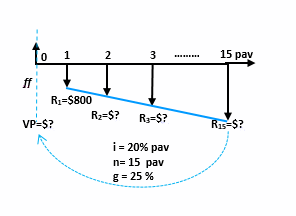
\includegraphics[height=5.0cm]{6_13(5)}
	\end{center}	    
		\item b. Declaración de variables\\
		R=\$800 \\ i = 20\% pav \\ g = 25\% de incremento entre serie geométrica con g $\not=$ i \\ n = 15 pav \\ VP= \$? \\ ff: en el período 0.\\
		\item c. Declaración de fórmulas\\
		$VP = \frac{R[(1+g)^n(1+i)^{-n}-1]}{g-i}$ \hspace{35 pt} \textit{Valor presente de una serie geométrica para g $\not=$ i}\\
		\item d. Desarrollo matemático:\\
		$VP = \frac{\$800[(1+0,25)^{15}(1+0,25)^{-15}-1]}{0,25-0,2}$ \hspace{35 pt} \textit{Ecuación de valor}\\
		\item e. Respuesta:\\
		Luego el valor presente es de VP = \$13.516\\
	\end{itemize}
	
	\textbf{Ejemplo 9}\\
	Elaborar una tabla para amortizar la suma de \$100.000 en 4 pagos, suponiendo una tasa del 8\% periódica anual vencida y:
	\begin{itemize}
		\item a. Crecimiento geométrico periódico de 10\% de los flujos
		\item b. Decrecimiento geométrico periódico de 10\% de los flujos
	\end{itemize}
	\textbf{Desarrollo caso a}
	\begin{itemize}
		\item a. Diagrama de flujo:\\
		\begin{center}
			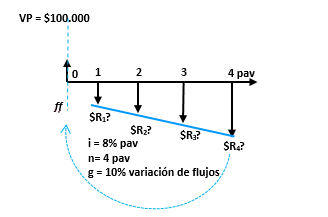
\includegraphics[height=5.5cm]{6_14}
		\end{center}
		\item b. Declaración de variables\\
		VP = \$100.000 \\		
		i = 8\% pav \\
		n = 4 pav \\
		g = 10\% creciente geométrico periódico\\
		g $\not=$ i\\
		
		\item c. Declaración de fórmulas\\
		Como g $\not = i$ entonces se emplea la fórmula \\
		$VF = \frac{R[((1+g)^n)((1+i)^{-n})-1]}{g-i}$ \hspace{35 pt} \textit{Valor futuro de gradiente geométrico para g $\not=$ i}\\ 
		$R_{n} = R_{1}(1+g)^{n-1}$ \hspace{20 pt} \textit{Valor del flujo n de gradiente geométrico}\\
		\item d.Desarrollo matemático\\
		$\$100.000 = \frac{R_{i}[((1+0,1)^{4})((1+0,08)^{-4}-1)]}{0,1-0,08}$ \hspace{35 pt} \textit{Ecuación de valor}\\
		\item e. Solución\\
		Donde\\
		$R_{1} = \$26.261,47$\\
		$R_{2} = \$26.261,47(1+0,1) = \$28.887,61$\\
		$R_{3} = \$26.261,47(1+0,1)^2 = \$31.776,38$\\
		$R_{4} = \$26.261,47(1+0,1)^3 = \$34.954,01 $\\
		
		
	\begin{spacing}{1.1}
    \begin{center}
        \begin{tabular}{|p{1cm}|p{2cm}|p{2.1cm}|p{2cm}|p{3cm}|}
        \hline 
        \rowcolor{white!50}
            \textbf{n\ (1)} & \textbf{Saldo Deuda (2)=(2)-(5)} & \textbf{Intereses  (3)=(2)(i)}& \textbf{Pago\ (4)=\$R-\$L }& \textbf{Amortización  (5)=(4)-(3)} \\ \hline                        

            0 & \$100.000,00 & --------- & --------- & ---------\\ \hline 
            1 & \$7.845,30  & \$1.000,00  & \$3.154,70  & \$2.154,70 \\ \hline
            2 & \$5.475,13  & \$784,53  & \$3.154,71  & \$2.370,17 \\ \hline
            3 & \$2.867,94 & \$547,51  & \$3.154,72 & \$2.607,19 \\ \hline
            4 & \$0,03  & \$286,79  & \$3.154,73  & \$2.867,91 \\ \hline
    \end{tabular}
    \end{center}
    \end{spacing}
    \end{itemize}
    
	\textbf{Desarrollo caso b}\\
	\begin{itemize}
	    \item a.Diagrama de flujo\\
	    \begin{center}
			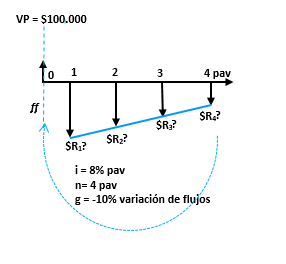
\includegraphics[height=6.5cm]{6_15}
		\end{center}
		\item b.Declaración de variables\\
		VP = \$100.000\\
		n = 4 pav\\
		g = -10\% decreciente \\
		i = 8\% pav\\
		g $\not=$ i\\
		
		\item c.Declaración de fórmulas\\
		Como $g\not= i$ entonces se emplea la fórmula\\
		$VF = \frac{R[((1+g)^n)((1+i)^{-n})-1]}{g-i}$ \hspace{35 pt} \textit{Valor futuro de gradiente geométrico para g $\not=$ i}\\
		$R_{n} = R_{1}(1+g)^{n-1}$ \hspace{35 pt} \textit{Valor del segundo flujo del gradiente geométrico}\\
		\item d.Desarrollo matemático\\
		\$100.000 = $\frac{R[((1-0,1)^4)((1+0,08)^{-4}-1)]}{-0,1-0,08}$ \hspace{35 pt} \textit{Ecuación de valor}\\
		\item e. Solución\\
		Donde se obtiene que:\\\\
		$R_{1} = \$34.766,02$\\
		$R_{2} = \$34.766.02(1-0,1) = \$31.289,42$\\
		$R_{3} = \$34.766,02(1-0,1)^2 = \$28.160,48$\\
		$R_{4} = \$34.766,02(1-0,1)^3 = \$25.344,43$\\\\\\
		Respuesta\\
		%\begin{center}
		%	\includegraphics[height=4.0cm]{}
		%\end{center}
		
	\begin{spacing}{1.1}
    \begin{center}
        \begin{tabular}{|p{1cm}|p{2cm}|p{2.1cm}|p{2cm}|p{3cm}|}
        \hline 
        \rowcolor{white!50}
            \textbf{n\ (1)} & \textbf{Saldo Deuda (2)=(2)-(5)} & \textbf{Intereses  (3)=(2)(i)}& \textbf{Pago\ (4)=\$R-\$L }& \textbf{Amortización  (5)=(4)-(3)} \\ \hline                     

            0 & \$100.000,00 & --------- & --------- & ---------\\ \hline 
            1 & \$7.845,30  & \$1.000,00  & \$3.154,70  & \$2.154,70 \\ \hline
            2 & \$5.475,13  & \$784,53  & \$3.154,71  & \$2.370,17 \\ \hline
            3 & \$2.867,94 & \$547,51  & \$3.154,72 & \$2.607,19 \\ \hline
            4 & \$0,03  & \$286,79  & \$3.154,73  & \$2.867,91 \\ \hline

 
\end{tabular}
\end{center}
\end{spacing}
	\end{itemize}
	
	\textbf{Ejemplo 10}\\
	¿Cuánto debe crecer linealmente una serie de 8 egresos efectuados al final de cada período y cuyo primer egreso es de \$600 para que, puesta en valor presente, sea equivalente a una serie de 10 egresos que crecen geométricamente en un 25\% y cuyo primer egreso es de \$100?. Suponga una tasa del 3\% periódica anual vencida.\\
	
	\textbf{Solución:}\\
	\begin{itemize}
		\item a.Diagrama de flujo:\\
		\begin{center}
			Deuda inicial\\
		\end{center}
		\begin{center}
			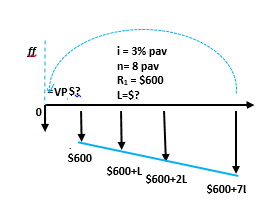
\includegraphics[height=5.0cm]{6_16}
		\end{center}
		\begin{center}
			Deuda equivalente\\
		\end{center}
		\begin{center}
			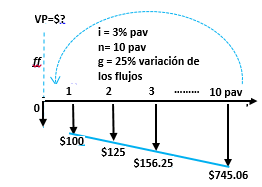
\includegraphics[height=5.0cm]{6_17}
		\end{center}
		\item b. Declaración de variables\\
	%	\begin{align*}
			$n_{1} = 8$ pav\\
			$n_{2} = 10$ pav\\
			$i = 3$\% pav\\
			$L = \$?$\\
			$R_{1} = $\$600\\
			$R_{2} = $\$100\\
			$g = 25$\% crecimiento geométrico periódico\\
			$g \not=$ i\\
	%	\end{align*}
		
		\item c. Declaración de fórmulas\\
		\\$VP=R\frac{(1+i)^n-i}{i}+\frac{L}{i}[\frac{(1+i)^n-i}{i}-n(1+i)^{-n}]$\hspace{20 pt} \textit{Valor presente de un gradiente aritmético}\\
		$VP = R\frac{(1+g)^n(1+i)^{-n}}{g-i}$ \hspace{35 pt} \textit{Valor presente de un gradiente geométrico si g $\not=$ i}\\
		\item d. Desarrollo matemático\\
		Debemos igualar el valor de las dos series y despejar L\\
		\\$VP = \$600\frac{1-(1+0,03)^{-8}}{0,03} + \frac{L}{0,03}[\frac{(1+0,03)^{-8}-1}{0,03}-8(1+0,03)^{-8}] = $ \hspace{35 pt} \textit{Ecuación de valor}\\
		$VP = \$100\frac{(1+0,25)^{10}(1+0,03)^{-10}-1}{0,25-0,03}$ \hspace{35 pt} \textit{Ecuación de valor}\\
		\item e. Respuesta:\\
		De donde se obtiene que L = \$-64,58, significa que el gradiente es decreciente, como se muestra en la gráfica:\\
		\begin{center}
			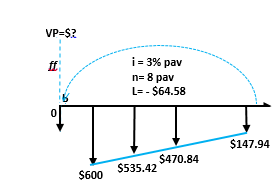
\includegraphics[height=5.0cm]{6_18}
		\end{center}
	\end{itemize}
	
	\textbf{Ejemplo 11}\\
	Se hacen depósitos trimestrales con incremento del 5\% entre flujos, en una cuenta que paga el 5,25\% periódica trimestral vencida, con el fin de tener disponibles \$500.000 el primero de enero de 1991. Si el primer depósito se hace el primero de abril de 1998 y el último el primero de julio de 1998. determinar el valor del primer depósito:\\
	
	\textbf{solución}\\
	\begin{itemize}
		\item a. Diagrama de flujo:\\
		\begin{center}
			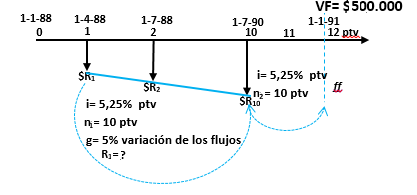
\includegraphics[height=5.0cm]{6_19}
		\end{center}
		\item b.Declaración de variables\\
	%	\begin{align*}
			VF= \$500.000\\
			R=\$?\\
			g = 5\% de incremento entre depósitos\\
			i= 5,25\% ptv\\
			$n_{1} = 10$ ptv\\
		$	n_{2} = 2$ ptv\\
			
	%	\end{align*}
		\item c. Declaración de formulas:\\
		
		$VF = R\frac{(1+g)^n-(1+i)^n}{g-i}$ \hspace{35 pt} \textit{Valor futuro gradiente si g $\not=$ i}\\
		$F = P(1+i)^n$ \hspace{35 pt} \textit{Valor futuro}\\
		\item d. Desarrollo matemático\\
		$\$500.000 = (\frac{R[(1+0,05)^{10}-(1+0,0525)^{10}]}{0,05-0,0525}*(1+0,0525)^2)$ \hspace{35 pt} \textit{Ecuación de valor}\\
		\item e. Respuesta:\\
		Despejando se obtiene que R = \$28.784,88 como primera cuota\\
	\end{itemize}
	
	\section{Gradiente geométrico infinito}
	Una de las aplicaciones que tiene este tipo de gradientes está en el análisis sobre emisión de acciones, que se estudiará en capítulos posteriores. Solo tiene sentido el análisis del valor presente.\\
	
	%formula VP
	\begin{center}
	\fontsize{13}{13}\selectfont
			$VP = \left \{ \begin{matrix}\frac{R}{i-g}& \mbox{si }g\mbox{ <  i}
 \\ \infty & \mbox{si }g\mbox{ >  i}\end{matrix}\right.$
	\end{center}

	
	\textbf{Ejemplo 12}\\
	Hallar el valor presente de una serie infinita de egresos que crecen en un 10\%, si la tasa de interés es del 20\% periódica anual vencida y el primer egreso es \$300.\\
	
	\textbf{Solución:}\\
	\begin{itemize}
		\item a. Diagrama de flujo:\\
		\begin{center}
			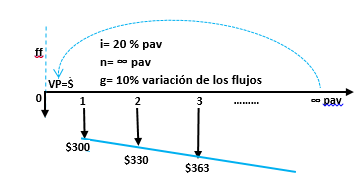
\includegraphics[height=4.8cm]{6_21}
		\end{center}
		\item b. Declaración de variables:\\
		n = $\infty$ \hspace{3 pt} pav\\
		$R_{1}$ = \$300\\
		g = 10\% creciente entre flujos\\
		i = 20\% pav\\
		VP = \$?\\
		\item c. Declaración de fórmulas:\\
		$VP = \frac{R}{i-g}$ \hspace{35 pt} \textit{Valor presente gradiente geométrico infinito si g<1}\\
		\item d. Desarrollo matemático\\
		$VP = \frac{\$300}{0,2-0,1} = \$3.000$ \hspace{35 pt} \textit{Ecuación de valor}\\
		\item e. Respuesta\\
		Significa que, si colocamos \$3000 al 20\% pav podremos hacer infinito número de retiros crecientes, en un 10\%, con un primer retiro de \$300.
	\end{itemize}
	
	\section{Gradientes escalonados}
	En este capitulo haremos una breve introducción al tema de los gradientes escalonados, pero en el siguiente capítulo, para poder analizar algunos sistemas de amortización, es necesario volver sobre este asunto y analizarlo con más detalle.\\
	
	Un gradiente escalonado es una serie de ingresos o egresos que permanecen constantes durante cierto tiempo, pero 	que crecen o decrecen periódicamente.\\
	
	Para trabajar con gradientes escalonados es más conveniente elaborar dos gráficas: en la primera, que denominaremos el gradiente escalonado, se colocan los ingresos o egresos en la misma forma en que van a ser pagadas las cuotas, y en la segunda gráfica que denominaremos el gradiente simple, se colocará el valor final de cada serie de ingresos o egresos iguales.\\
	
	En la primera gráfica a todos los datos tales como ingresos o egresos, tasa y período se les antepone  el prefijo sub o ínter así: ínter-pago o ínter-cuota, inter-tasa e inter-período, en la segunda gráfica no habrá cambios.\\
	
	Normalmente sólo se da la información de una de las dos tasas bien sea la inter-tasa o la tasa, lo importante es que la que no se conoce se puede calcular a partir de la que se conoce mediante la equivalencia de tasas.\\
	
	Representaremos por m el número de inter-cuotas por cada cuota y se le denominará tamaño de escalón.\\
	
	Se recomienda que al frente de cada dibujo se coloquen los respectivos datos a fin de evitar confusiones.\\
	
	\textbf{Ejemplo 13}\\
	Supongamos que se va a reunir \$800.000 mediante depósitos mensuales durante 5 años, con la siguiente condición: los depósitos durante el primer año son iguales; para comenzar el segundo año aumentan un 15\% y permanecerán constantes durante ese mismo año: al comenzar el tercer año vuelven a subir otro 15\% y permanecen constantes durante ese año y así sucesivamente.\\
	Con una tasa del 27\% periódica anual vencida: calcular el valor del primer depósito y el valor del último depósito del gradiente escalonado.\\
	
	\textbf{Solución:}\\
	\begin{itemize}
		\item a. Diagrama de flujo:
		\begin{center}
			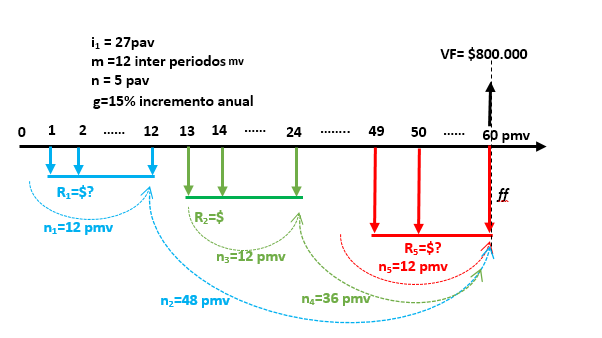
\includegraphics[height=6.0cm]{6_22}
		\end{center}
		\item b. Declaración de variables\\
		\\VF = \$800.000\\
		$R_{1}$ = \$? primer intercuota\\
		$R_{60}$ = \$? última intercuota\\
		$n_{1} = 5$ pav equivalente a 60 pmv de interperíodos\\
        $n_{2} =  12$ inter períodos mes vencido\\ 	
		i simple = $i_{1}= 27$\% pav\\
		i intertasa = $i_{2}= ?$\% pmv\\
		g = 15\% incremento entre depósitos anual\\\\
		\item c. Declaración de fórmulas\\\\
		$(1+i_{1})^{m_{1}} = (1+i_{2})^{m_{2}}$ \hspace{31 pt} \textit{Equivalencia de tasas}\\
		$VF = R\frac{(1+g)^n-(1+i)^n}{g-i}$ \hspace{38 pt} \textit{Valor futuro gradiente geométrico si g $\not=$ i}\\
		$R_{n} = R_{n-1}(1+g)^{n-1}$ \hspace{35 pt} \textit{Flujo de un gradiente geométrico}\\
		$VF = R\frac{(1+i)^{n}-1}{i}$ \hspace{56 pt} \textit{VF de una serie uniforme}\\
		\item d. Desarrollo matemático\\\\
		$(1+i_{1})^1 = (1+i_{2})^{12}$
		$(1+0,27)^1 = (1+i_{2})^{12}$\\\\ Despejando se obtiene: \\
		$i_{2} = 2.01178$\% pmv, equivalente a la intertasa pav.\\
		\begin{center}
			\textbf{Diagrama de flujo de la serie simple}\\
		\end{center}
		\begin{center}
			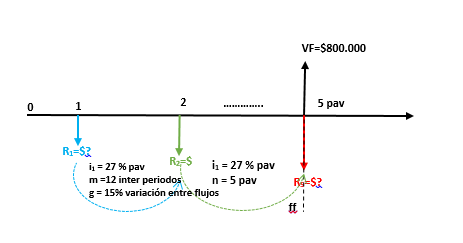
\includegraphics[height=5.0cm]{6_23}
		\end{center}
		Primero comenzamos los cálculos con el gradiente simple y hallamos el valor de las cuotas $R_{1}$ y  $R_{5}$\\\\
		$\$800.000 = \frac{R[(1.15)^5-(1,27)^5]}{0,15-0,27}$ \hspace{35 pt} \textit{Ecuación de valor \\\\ $n_{1}$ = 5 períodos anuales vencidos; $i_{1}$ = 27\% pav; g = 15\% de aumento ente flujos}\\
		De donde se obtiene que $ R_{1}$ = \$ 74.275,83 y el valor de $R_{5} = 74.275,83(1 + 0,15)^{4} = \$129.908,88$\\\\
		Ahora pasamos al gradiente escalonado determinando las intercuotas, los interperíodos y observamosque el valor final de las 12 primeras cuotas (que son del mismo valor) debe ser igual a la primera cuota del gradiente simple.\\\\
		intertasa = $i_{2}$ = 2,01178\% pmv\\
		interperíodo = $n_{2}$ = 12 pmv\\
		interflujo año 1 = $R_{1}$ = \$? \\
		interflujo año 2 = $R_{2}$ = \$? \\
		interflujo año 3 = $R_{3}$ = \$? \\
		interflujo año 4 = $R_{4}$ = \$? \\
		interflujo año 5 = $R_{5}$ = \$? \\\\
		
	Utilizando la fórmula del valor futuro de una serie uniforme se procede a calcular $R_{1} y  R_{60}$ de una serie escalonada\\\\
        		
		$\$74.275,83 = R_{1}\frac{(1+0.02)^{12}-1}{0.02}$\\
		
		
		$R_{1} = \$5.537,97$\\\\
		En igual forma la última cuota se podrá calcular así:\\
		
		$ \$129.908,88 = R_{60}\frac{(1,02)^{12}-1}{0.02}$\\\\
		$R_{60} = \$9.685,95$\\
		\item e. Solución\\
	
	\textbf{	$R_{1} = \$5.537,97$ y $R_{60} = \$9.685,95$}\\\\
		\textbf{Observación:} Cuando se quiere calcular el valor final o el valor presente de todo el gradiente escalonado se puede calcular mediante la segunda gráfica, es decir, que se calcula el gradiente simple.
		
	\end{itemize}
	
	
	%----------------------------------------------------------------------------------------
	%	PART
	%----------------------------------------------------------------------------------------
	
	%\part{Parte Dos}
	
	%----------------------------------------------------------------------------------------
	%	CHAPTER 3
	%----------------------------------------------------------------------------------------
	
	%\chapterimage{ima2} % Chapter heading image
	
	
	%Anexos
	%\chapter*{Anexos}
	%\addcontentsline{toc}{chapter}{\textcolor{ocre}{Anexos}}
	
	
	
	
	%----------------
	
	%----------------------------------------------------------------------------------------
	%	BIBLIOGRAPHY
	%----------------------------------------------------------------------------------------
	
	%\chapter*{Bibliografía}
	%\addcontentsline{toc}{chapter}{\textcolor{ocre}{Bibliografía}}
	%\section*{Books}
	%\addcontentsline{toc}{section}{Books}
	%\printbibliography[heading=bibempty,type=book]
	
	
	
	%----------------------------------------------------------------------------------------
	%	INDEX
	%----------------------------------------------------------------------------------------
	
	\cleardoublepage
	\phantomsection
	\setlength{\columnsep}{0.75cm}
	\printindex
	
	%---------------------
